\chapter{Hilbert Complexes}\label{cha:Hilbert complexes}
    Define the following Hilbert spaces and exact complexes:
    
    \section{1D in Time}
         On $T^{k}$:
        
        \subsection*{$H\Lambda^{\bullet}\left(T^{k}\right)$}
            Define the Hilbert spaces: \BA{(I haven't really defined what norms these spaces use... Not sure I need to really though...)}
            \begin{align}
                L^{2}  :=  \left\{u \in L^{1}_{\rm loc} : \|u\|_{T^{k}} < \infty\right\},  &&
                H^{1}  :=  \left\{u \in L^{1}_{\rm loc} : \partial_{t}u \in L^{2}\right\}
            \end{align}
            Define the exact complex $H\Lambda^{\bullet}\left(T^{k}\right)$:
            \begin{center}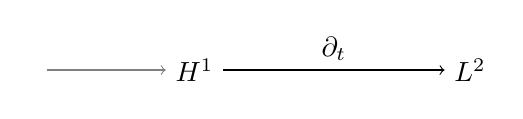
\begin{tikzpicture}[align = center, node distance = 4cm, auto]
                \node (R)  at (- 2, 0) {\color{black!50} $\bbR$};
                \node (H1) at (0,   0) {$H^{1}$};
                \node (L2) at (3.5, 0) {$L^{2}$};
    
                \draw[->, draw = black!50] (R)  -- (H1);
                \draw[->] (H1) -- (L2) node[above, midway] {$\partial_{t}$};
            \end{tikzpicture}\end{center}

        \subsection*{$H_{0}\Lambda^{\bullet}\left(T^{k}\right)$}
            Define the Hilbert space:
            \begin{equation}
                H^{1}_{0}  :=  \left\{u \in H^{1} : u = 0|_{t \in \partial T^{k}}\right\}
            \end{equation}
            Define the exact complex $H_{0}\Lambda^{\bullet}\left(T^{k}\right)$:
            \begin{center}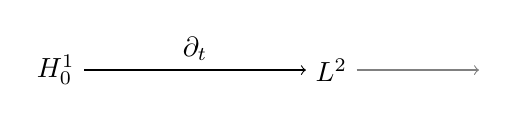
\begin{tikzpicture}[align = center, node distance = 4cm, auto]
                \node (H1) at (0,   0) {$H^{1}_{0}$};
                \node (L2) at (3.5, 0) {$L^{2}$};
                \node (R)  at (5.5, 0) {\color{black!50} $\bbR$};
    
                \draw[->] (H1) -- (L2) node[above, midway] {$\partial_{t}$};
                \draw[->, draw = black!50] (L2) -- (R);
            \end{tikzpicture}\end{center}

        \subsection*{$H_{\pm}\Lambda^{\bullet}\left(T^{k}\right)$}
            Define the Hilbert spaces:
            \begin{align}
                H^{1}_{+}  :=  \left\{u \in H^{1} : u = 0|_{t = t^{k + 1}}\right\},  &&
                H^{1}_{-}  :=  \left\{u \in H^{1} : u = 0|_{t = t^{k}}\right\}
            \end{align}
            Define the exact complexes $H_{\pm}\Lambda^{\bullet}(\bfOmega)$:
            \begin{center}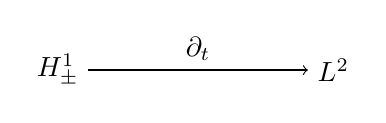
\begin{tikzpicture}[align = center, node distance = 4cm, auto]
                \node (H1) at (0,   0) {$H^{1}_{\pm}$};
                \node (L2) at (3.5, 0) {$L^{2}$};
    
                \draw[->] (H1) -- (L2) node[above, midway] {$\partial_{t}$};
            \end{tikzpicture}\end{center}
        
    \section{3D in Space}
        On $\bfOmega$:

        \subsection*{$H\Lambda^{\bullet}(\bfOmega)$}
            Define the Hilbert spaces: \BA{(Bit of a clash in notation here on the $L^{2}$'s.)}
            \begin{align}
                L^{2}          &:=  \left\{u \in L^{1}_{\rm loc} : \|u\|_{\bfOmega} < \infty\right\}  \\
                \bfH(\rmdiv)   &:=  \left\{\bfu \in \left(L^{1}_{\rm loc}\right)^{3} : \nabla\cdot\bfu \in L^{2}\right\}  \\
                \bfH(\bfcurl)  &:=  \left\{\bfu \in \left(L^{1}_{\rm loc}\right)^{3} : \nabla\wedge\bfu \in \left(L^{2}\right)^{3}\right\}  \\
                H^{1}          &:=  \left\{u \in L^{1}_{\rm loc} : \nabla u \in \left(L^{2}\right)^{3}\right\}
            \end{align}
            Define the exact complex of vector proxies for $H\Lambda^{\bullet}(\bfOmega)$: \BA{([Ref])}
            \begin{center}\begin{tikzpicture}[align = center, node distance = 4cm, auto]
                \node (R)     at (- 2,  0) {\color{black!50} $\bbR$};
                \node (H1)    at (0,    0) {$H^{1}$};
                \node (Hcurl) at (3.5,  0) {$\bfH(\bfcurl)$};
                \node (Hdiv)  at (7,    0) {$\bfH(\rmdiv)$};
                \node (L2)    at (10.5, 0) {$L^{2}$};
    
                \draw[->, draw = black!50] (R) -- (H1);
                \draw[->] (H1)    -- (Hcurl) node[above, midway] {$\bfgrad$};
                \draw[->] (Hcurl) -- (Hdiv)  node[above, midway] {$\bfcurl$};
                \draw[->] (Hdiv)  -- (L2)    node[above, midway] {$\rmdiv$};
            \end{tikzpicture}\end{center}

        \subsection*{$H_{0}\Lambda^{\bullet}(\bfOmega)$}
            Define the Hilbert spaces:
            \begin{align}
                \bfH_{0}(\rmdiv)   &:=  \left\{\bfu \in \bfH(\rmdiv) : \bfu\cdot\bfn = 0|_{\bfGamma}\right\}  \\
                \bfH_{0}(\bfcurl)  &:=  \left\{\bfu \in \bfH(\bfcurl) : \bfu\wedge\bfn = \bfzero|_{\bfGamma}\right\}  \\
                H^{1}_{0}          &:=  \left\{u \in H^{1} : u = 0|_{\bfGamma}\right\}
            \end{align}
            Define the exact complex of vector proxies for $H_{0}\Lambda^{\bullet}(\bfOmega)$: \BA{([Ref])}
            \begin{center}\begin{tikzpicture}[align = center, node distance = 4cm, auto]
                \node (H1)    at (0,    0) {$H^{1}_{0}$};
                \node (Hcurl) at (3.5,  0) {$\bfH_{0}(\bfcurl)$};
                \node (Hdiv)  at (7,    0) {$\bfH_{0}(\rmdiv)$};
                \node (L2)    at (10.5, 0) {$L^{2}$};
                \node (R)     at (12.5, 0) {\color{black!50} $\bbR$};
    
                \draw[->] (H1)    -- (Hcurl) node[above, midway] {$\bfgrad$};
                \draw[->] (Hcurl) -- (Hdiv)  node[above, midway] {$\bfcurl$};
                \draw[->] (Hdiv)  -- (L2)    node[above, midway] {$\rmdiv$};
                \draw[->, draw = black!50] (L2) -- (R);
            \end{tikzpicture}\end{center}
            
        \subsection*{$H_{\bfgamma}\Lambda^{\bullet}(\bfOmega)$}
            For $\bfgamma  \subseteq  \bfGamma$, define the Hilbert spaces:
            \begin{align}
                \bfH_{\bfgamma}(\rmdiv)   &:=  \left\{\bfu \in \bfH(\rmdiv) : \bfu\cdot\bfn = 0|_{\bfgamma}\right\}  \\
                \bfH_{\bfgamma}(\bfcurl)  &:=  \left\{\bfu \in \bfH(\bfcurl) : \bfu\wedge\bfn = \bfzero|_{\bfgamma}\right\}  \\
                H^{1}_{\bfgamma}          &:=  \left\{u \in H^{1} : u = 0|_{\bfgamma}\right\}
            \end{align}
            Define the complex of vector proxies for $H_{\bfgamma}\Lambda^{\bullet}(\bfOmega)$, exact if and only if $\bfgamma  \neq  \emptyset, \bfGamma$: \BA{([Ref])}
            \begin{center}\begin{tikzpicture}[align = center, node distance = 4cm, auto]
                \node (H1)    at (0,    0) {$H^{1}_{\bfgamma}$};
                \node (Hcurl) at (3.5,  0) {$\bfH_{\bfgamma}(\bfcurl)$};
                \node (Hdiv)  at (7,    0) {$\bfH_{\bfgamma}(\rmdiv)$};
                \node (L2)    at (10.5, 0) {$L^{2}$};
                
                \draw[->] (H1)    -- (Hcurl) node[above, midway] {$\bfgrad$};
                \draw[->] (Hcurl) -- (Hdiv)  node[above, midway] {$\bfcurl$};
                \draw[->] (Hdiv)  -- (L2)    node[above, midway] {$\rmdiv$};
            \end{tikzpicture}\end{center}
        
    \section{(3+1)D in Space and Time}
        \BA{Talk about tensor product subcomplexes.}
        
        On $\bfOmega\otimes T^{k}$:

        \subsection*{$H\Lambda^{\bullet}\left(\bfOmega\otimes T^{k}\right)$}
            Define the Hilbert spaces:
            \begin{align}
                L^{2}  &:=  \left\{u \in L^{1}_{\rm loc} : \|u\|_{\bfOmega\otimes T^{k}} < \infty\right\}  \\
                \bfH(\rmdiv + \partial_{t})  &:=  \left\{\begin{pmatrix} \bfu \\ v \end{pmatrix} \in \left(L^{1}_{\rm loc}\right)^{3 + 1} : \nabla\cdot\bfu + \partial_{t}v \in L^{2}\right\}  \\
                \bfH\left(\begin{matrix} \bfcurl + \partial_{t} \\ * - \rmdiv \end{matrix}\right)  &:=  \left\{\begin{pmatrix} \bfu \\ \bfv \end{pmatrix} \in \left(L^{1}_{\rm loc}\right)^{3 + 3} : \begin{pmatrix} \nabla\wedge\bfu + \partial_{t}\bfv \\ - \nabla\cdot\bfv \end{pmatrix} \in \left(L^{2}\right)^{3 + 1}\right\}  \\
                \bfH\left(\begin{matrix} - \bfgrad - \partial_{t} \\ * + \bfcurl \end{matrix}\right)  &:=  \left\{\begin{pmatrix} u \\ \bfv \end{pmatrix} \in \left(L^{1}_{\rm loc}\right)^{1 + 3} : \begin{pmatrix} - \nabla u - \partial_{t}\bfv \\ \nabla\wedge\bfv \end{pmatrix} \in \left(L^{2}\right)^{3 + 3}\right\}  \\
                H^{1}  &:=  \left\{v \in L^{1}_{\rm loc} : \begin{pmatrix} - \partial_{t}v \\ \nabla v \end{pmatrix} \in \left(L^{2}\right)^{1 + 3}\right\}
            \end{align}
            Define the exact complex of vector proxies for $H\Lambda^{\bullet}\left(\bfOmega\otimes T^{k}\right)$: \BA{([Ref])}
            {\scriptsize \begin{center}\begin{tikzpicture}[align = center, node distance = 4cm, auto]
                \node (R)   at (- 1.5, 0) {\color{black!50} $\bbR$};
                \node (HL0) at (0,     0) {$H^{1}$};
                \node (HL1) at (3,     0) {$\bfH\left(\begin{matrix} - \bfgrad - \partial_{t} \\ * + \bfcurl \end{matrix}\right)$};
                \node (HL2) at (7.5,   0) {$\bfH\left(\begin{matrix} \bfcurl + \partial_{t} \\ * - \rmdiv \end{matrix}\right)$};
                \node (HL3) at (11.5,  0) {$\bfH(\rmdiv + \partial_{t})$};
                \node (HL4) at (14,    0) {$L^{2}$};

                \draw[->, black!50] (R) -- (HL0);
                \draw[->] (HL0) -- (HL1) node[above, midway] {$\left(\begin{matrix} - \partial_{t} \\ \bfgrad \end{matrix}\right)$};
                \draw[->] (HL1) -- (HL2) node[above, midway] {$\left(\begin{matrix} - \bfgrad - \partial_{t} \\ * + \bfcurl \end{matrix}\right)$};
                \draw[->] (HL2) -- (HL3) node[above, midway] {$\left(\begin{matrix} \bfcurl + \partial_{t} \\ * - \rmdiv \end{matrix}\right)$};
                \draw[->] (HL3) -- (HL4) node[above, midway] {$\rmdiv + \partial_{t}$};
            \end{tikzpicture}\end{center}}

        \subsection*{$H_{0}\Lambda^{\bullet}\left(\bfOmega\otimes T^{k}\right)$}
            Define the Hilbert spaces:
            \begin{align}
                \bfH_{0}(\rmdiv + \partial_{t})  &:=  \left\{\begin{pmatrix} \bfu \\ v \end{pmatrix} \in \bfH(\rmdiv + \partial_{t}) : \bfu\cdot\bfn|_{\bfGamma\otimes T^{k}}, v|_{\bfOmega\otimes\partial T^{k}} = 0\right\}  \\
                \bfH_{0}\left(\begin{matrix} \bfcurl + \partial_{t} \\ * - \rmdiv \end{matrix}\right)  &:=  \left\{\begin{pmatrix} \bfu \\ \bfv \end{pmatrix} \in \bfH\left(\begin{matrix} \bfcurl + \partial_{t} \\ * - \rmdiv \end{matrix}\right) : \begin{matrix} \bfu\wedge\bfn|_{\bfGamma\otimes T^{k}}, \bfv|_{\bfOmega\otimes\partial T^{k}} = \bfzero \\ \bfv\cdot\bfn|_{\bfGamma\otimes T^{k}} = 0 \end{matrix}\right\}  \\
                \bfH_{0}\left(\begin{matrix} - \bfgrad - \partial_{t} \\ * + \bfcurl \end{matrix}\right)  &:=  \left\{\begin{pmatrix} u \\ \bfv \end{pmatrix} \in \bfH\left(\begin{matrix} - \bfgrad - \partial_{t} \\ * + \bfcurl \end{matrix}\right) : \begin{matrix} u|_{\bfGamma\otimes T^{k}} = 0, \bfv|_{\bfOmega\otimes\partial T^{k}} = \bfzero \\ \bfv\wedge\bfn|_{\bfGamma\otimes T^{k}} = \bfzero \end{matrix}\right\}  \\
                H^{1}_{0}  &:=  \left\{v \in H^{1} : \begin{matrix} v = 0|_{\bfOmega\otimes\partial T^{k}} \\ v = 0|_{\bfGamma\otimes T^{k}} \end{matrix}\right\}
            \end{align}
            Define the exact complex of vector proxies for $H_{0}\Lambda^{\bullet}\left(\bfOmega\otimes T^{k}\right)$: \BA{([Ref])}
            {\scriptsize \begin{center}\begin{tikzpicture}[align = center, node distance = 4cm, auto]
                \node (HL0) at (0,    0) {$H^{1}_{0}$};
                \node (HL1) at (3,    0) {$\bfH_{0}\left(\begin{matrix} - \bfgrad - \partial_{t} \\ * + \bfcurl \end{matrix}\right)$};
                \node (HL2) at (7.5,  0) {$\bfH_{0}\left(\begin{matrix} \bfcurl + \partial_{t} \\ * - \rmdiv \end{matrix}\right)$};
                \node (HL3) at (11.5, 0) {$\bfH_{0}(\rmdiv + \partial_{t})$};
                \node (HL4) at (14,   0) {$L^{2}_{0}$};
                \node (R)   at (15.5, 0) {\color{black!50} $\bbR$};
    
                \draw[->] (HL0) -- (HL1) node[above, midway] {$\left(\begin{matrix} - \partial_{t} \\ \bfgrad \end{matrix}\right)$};
                \draw[->] (HL1) -- (HL2) node[above, midway] {$\left(\begin{matrix} - \bfgrad - \partial_{t} \\ * + \bfcurl \end{matrix}\right)$};
                \draw[->] (HL2) -- (HL3) node[above, midway] {$\left(\begin{matrix} \bfcurl + \partial_{t} \\ * - \rmdiv \end{matrix}\right)$};
                \draw[->] (HL3) -- (HL4) node[above, midway] {$\rmdiv + \partial_{t}$};
                \draw[->, draw = black!50] (HL4) -- (R);
            \end{tikzpicture}\end{center}}

        \subsection*{$H_{\bfgamma\bfomega}\Lambda^{\bullet}\left(\bfOmega\otimes T^{k}\right)$}
            For $\bfgamma  \subseteq  \bfGamma\otimes T^{k}$, $\bfomega  \subseteq  \bfOmega\otimes\partial T^{k}$, define the Hilbert spaces:
            \begin{align}
                \bfH_{\bfgamma\bfomega}(\rmdiv + \partial_{t})  &:=  \left\{\begin{pmatrix} \bfu \\ v \end{pmatrix} \in \bfH(\rmdiv + \partial_{t}) : \bfu\cdot\bfn|_{\bfgamma}, v|_{\bfomega} = 0\right\}  \\
                \bfH_{\bfgamma\bfomega}\left(\begin{matrix} \bfcurl + \partial_{t} \\ * - \rmdiv \end{matrix}\right)  &:=  \left\{\begin{pmatrix} \bfu \\ \bfv \end{pmatrix} \in \bfH\left(\begin{matrix} \bfcurl + \partial_{t} \\ * - \rmdiv \end{matrix}\right) : \begin{matrix} \bfu\wedge\bfn|_{\bfgamma}, \bfv|_{\bfomega} = \bfzero \\ \bfv\cdot\bfn|_{\bfgamma} = 0 \end{matrix}\right\}  \\
                \bfH_{\bfgamma\bfomega}\left(\begin{matrix} - \bfgrad - \partial_{t} \\ * + \bfcurl \end{matrix}\right)  &:=  \left\{\begin{pmatrix} u \\ \bfv \end{pmatrix} \in \bfH\left(\begin{matrix} - \bfgrad - \partial_{t} \\ * + \bfcurl \end{matrix}\right) : \begin{matrix} u\bfn|_{\bfgamma}, \bfv|_{\bfomega} = \bfzero \\ \bfv\wedge\bfn|_{\bfgamma} = \bfzero \end{matrix}\right\}  \\
                H^{1}_{\bfgamma\bfomega}  &:=  \left\{v \in H^{1} : \begin{matrix} v = 0|_{\bfomega} \\ v = 0|_{\bfgamma} \end{matrix}\right\}
            \end{align}
            Define the complex of vector proxies for $H_{\pm}\Lambda^{\bullet}\left(\bfOmega\otimes T^{k}\right)$, exact if and only if $\bfgamma\cup\bfomega  \neq  \emptyset, \partial\left(\bfOmega\otimes T^{k}\right)  \left(=  \left(\bfGamma\otimes T^{k}\right)\cup\left(\bfOmega\otimes\partial T^{k}\right)\right)$: \BA{([Ref])}
            {\scriptsize \begin{center}\begin{tikzpicture}[align = center, node distance = 4cm, auto]
                \node (HL0) at (0,    0) {$H^{1}_{\bfgamma\bfomega}$};
                \node (HL1) at (3,    0) {$\bfH_{\bfgamma\bfomega}\left(\begin{matrix} - \bfgrad - \partial_{t} \\ * + \bfcurl \end{matrix}\right)$};
                \node (HL2) at (7.5,  0) {$\bfH_{\bfgamma\bfomega}\left(\begin{matrix} \bfcurl + \partial_{t} \\ * - \rmdiv \end{matrix}\right)$};
                \node (HL3) at (11.5, 0) {$\bfH_{\bfgamma\bfomega}(\rmdiv + \partial_{t})$};
                \node (HL4) at (14,   0) {$L^{2}$};
    
                \draw[->] (HL0) -- (HL1) node[above, midway] {$\left(\begin{matrix} - \partial_{t} \\ \bfgrad \end{matrix}\right)$};
                \draw[->] (HL1) -- (HL2) node[above, midway] {$\left(\begin{matrix} - \bfgrad - \partial_{t} \\ * + \bfcurl \end{matrix}\right)$};
                \draw[->] (HL2) -- (HL3) node[above, midway] {$\left(\begin{matrix} \bfcurl + \partial_{t} \\ * - \rmdiv \end{matrix}\right)$};
                \draw[->] (HL3) -- (HL4) node[above, midway] {$\rmdiv + \partial_{t}$};
            \end{tikzpicture}\end{center}}
        
            \line
            
            \begin{lemma}
                For $\bfgamma  \subseteq  \bfGamma$, with tensor product complexes as defined in \cite{ABB15} (and ignoring the presence of $\bbR$ in the sequence when included for exactness):
                \begin{align}
                    H_{\bfgamma}\Lambda^{\bullet}(\bfOmega)\otimes H\Lambda^{\bullet}\left(T^{k}\right)  &<  H_{\bfgamma\otimes T^{k}, \emptyset}\Lambda^{\bullet}\left(\bfOmega\otimes T^{k}\right)  \\
                    H_{\bfgamma}\Lambda^{\bullet}(\bfOmega)\otimes H_{0}\Lambda^{\bullet}\left(T^{k}\right)  &<  H_{\bfgamma\otimes T^{k}, \bfOmega\otimes\partial T^{k}}\Lambda^{\bullet}\left(\bfOmega\otimes T^{k}\right)  \\
                    H_{\bfgamma}\Lambda^{\bullet}(\bfOmega)\otimes H_{+}\Lambda^{\bullet}\left(T^{k}\right)  &<  H_{\bfgamma\otimes T^{k}, \bfOmega\otimes\{T\}}\Lambda^{\bullet}\left(\bfOmega\otimes T^{k}\right)  \\
                    H_{\bfgamma}\Lambda^{\bullet}(\bfOmega)\otimes H_{-}\Lambda^{\bullet}\left(T^{k}\right)  &<  H_{\bfgamma\otimes T^{k}, \bfOmega\otimes\{0\}}\Lambda^{\bullet}\left(\bfOmega\otimes T^{k}\right)
                \end{align}
                where the subcomplex inclusion is \emph{proper}.
            \end{lemma}

            \begin{corollary}\label{cor:tensor product complex inclusion}
                \begin{align}
                    H\Lambda^{\bullet}(\bfOmega)\otimes H\Lambda^{\bullet}\left(T^{k}\right)  &<  H\Lambda^{\bullet}\left(\bfOmega\otimes T^{k}\right)  \\
                    H_{0}\Lambda^{\bullet}(\bfOmega)\otimes H_{0}\Lambda^{\bullet}\left(T^{k}\right)  &<  H_{0}\Lambda^{\bullet}\left(\bfOmega\otimes T^{k}\right)
                \end{align}
                where the subcomplex inclusion is \emph{proper}.
            \end{corollary}

            \line
    